\documentclass[a4paper]{jlreq}
\usepackage[haranoaji]{luatexja-preset}

\usepackage{amsmath, amssymb}
\usepackage{bm}
\usepackage{siunitx}
\usepackage{listings}

\usepackage{graphicx}
\usepackage{svg}
\usepackage{wrapfig}

\begin{document}
  \title{document}
  \author{Actat}
  \date{}
  \maketitle

  \section{ロボット製作の動機}

  このロボットの製作に取り組むのは,歩行ロボット製作を経験するためである.
  最終的には二足歩行ロボットの製作を目指しているが,6自由度の脚の設計は難易度が高いと判断し,
  今回は3自由度の脚を4つ備えた四足歩行ロボットを製作することにした.

  このロボットの製作では以下の内容を経験することを期待している.
  \begin{itemize}
    \item 自宅でのロボット製作
    \item サーボモータを用いた機構の設計
    \item 最低限の電気回路の取扱い
    \item ROSを用いたプログラミング
    \item 歩行ロボットの制御
  \end{itemize}

  \section{機械設計・製作}

  設計・製作したロボットを図\ref{fig:robot}に示す.
  脚は前後左右に鏡像になっている同一の機構とした.
  サーボモータは研究室で使用しているモータと合わせて近藤科学株式会社のB3M-SC-1170-Aを用いた.
  CIT Brainsが公開しているB3Mモータを用いた二足歩行ロボットを参考に,関節間の距離は\SI{100}{mm}にした.

  胴体中央下部に株式会社アールティのUSB出力9軸IMUセンサモジュールを搭載した.
  センサの位置をロボットのベースリンクと一致させて計算を簡単にする意図がある.
  胴体上部前方に取り付けられた板にサーボモータとPCの間の通信のための基板を固定した.

  \begin{figure}[htb]
    \centering
    \input{robot.pdf_tex}
    \caption{
      設計・製作したロボット
    }
    \label{fig:robot}
  \end{figure}

  \section{電装}

  ロボット全体で12個のモータが使われている.
  モータとパソコンはRS485USB/シリアル変換アダプターを介して通信する.
  直列に接続できるモータの数は限られているので
  XHコネクター用ハブ typeAによって各脚ごとの系統に分けて接続した.
  配線の様子を図\ref{fig:wiring}に示す.

  XHコネクター用ハブには5つのコネクタがあり,すべて並列に接続される.
  このハブはロボット前方に横向きに取り付けられており,
  中央のコネクタをRS485USB/シリアル変換アダプターに接続し,
  左右のコネクタをそれぞれ脚のモータと接続した.
  脚の3つのモータはHip flexion/extension, Hip ab/adduction, kneeの順に接続された.
  Hipのモータは機械的な接続とは逆の順序である.

  \begin{figure}[htb]
    \centering
    \input{wiring.pdf_tex}
    \caption{
      配線の様子
    }
    \label{fig:wiring}
  \end{figure}

  サーボモータは配線に先立ってIDの書き込みを行った.
  書き込んだIDは表\ref{table:servo_id}に示すとおりである.

  \begin{table}[htb]
    \caption{IDと関節の対応}
    \label{table:servo_id}
    \centering
    \begin{tabular}{rcc}
      \hline
      id & 脚 & 関節 \\
      \hline
      0 & 左前 & Hip ab/adduction \\
      1 & 左前 & Hip flexion/extension \\
      2 & 左前 & knee \\
      3 & 右前 & Hip ab/adduction \\
      4 & 右前 & Hip flexion/extension \\
      5 & 右前 & knee \\
      6 & 左後 & Hip ab/adduction \\
      7 & 左後 & Hip flexion/extension \\
      8 & 左後 & knee \\
      9 & 右後 & Hip ab/adduction \\
      10 & 右後 & Hip flexion/extension \\
      11 & 右後 & knee \\
      \hline
    \end{tabular}
  \end{table}

  \section{Packageの作成}

  別のディレクトリで
  \texttt{\$ ros2 pkg create --build-type ament\_cmake --node-name quadruped\_takahashi quadruped\_takahashi}
  を実行してpackage.xml, CMakeLists.txt, quadruped\_takahashi.cppを作成した.
  その後,作成したファイルをこのリポジトリ内へ移動した.

  \section{モータとの通信}

  モータとの通信にはActat/kondo\_b3m\_ros2を用いる.
  remakeブランチ\footnote{このプロジェクトでうまく動作することを確認したらmasterにする予定である.}に合わせて
  launchファイルを用意し,通信ができることを確認する.
  以下にlaunchファイルのうち,kondo\_b3m\_ros2のノードの設定に関する部分を抜粋する.
  軸の方向を反転しているのは,後述する座標系に合わせるためである.

  \begin{lstlisting}[basicstyle=\ttfamily, language=Python]
    kondo_b3m_ros2_node = Node(
      package='kondo_b3m_ros2',
      executable='kondo_b3m',
      remappings=[('b3m_joint_state', 'joint_states')],
      parameters=[{'motor_list': [
        "{'id': 0, 'name': 'lf0', 'direction': False}",
        "{'id': 1, 'name': 'lf1', 'direction': False}",
        "{'id': 2, 'name': 'lf2', 'direction': False}",
        "{'id': 3, 'name': 'rf0', 'direction': False}",
        "{'id': 4, 'name': 'rf1'}",
        "{'id': 5, 'name': 'rf2'}",
        "{'id': 6, 'name': 'lh0'}",
        "{'id': 7, 'name': 'lh1', 'direction': False}",
        "{'id': 8, 'name': 'lh2', 'direction': False}",
        "{'id': 9, 'name': 'rh0'}",
        "{'id': 10, 'name': 'rh1'}",
        "{'id': 11, 'name': 'rh2'}"
      ]}],
    )
  \end{lstlisting}

  あるウインドウで\texttt{\$ ros2 launch quadruped\_takahashi launch.py}を実行して起動し,
  別のウインドウで\texttt{\$ ros2 topic echo /joint\_states}することで各関節の角度・角速度が出力されていることを確認した.

  \section{URDFファイルの作成}

  URDFファイルの作成にあたってロボットの関節に関する座標系を設定する.
  初めに左前脚を考える(図\ref{fig:lfleg_coords}).
  2つのHipの関節は軸が交わるように作られており,この交点を脚の付け根とする.
  脚の付け根を原点としてロボットの前方に$x$軸,左方向に$y$軸,鉛直上方向に$z$軸をとった座標系を$\Sigma_\mathrm{lf0}$とする.
  $\Sigma_\mathrm{lf0}$の$x$軸はHip ab/adductionの関節軸と一致しており,
  この軸周りに$\theta_\mathrm{lf0}$回転した座標系を$\Sigma_\mathrm{lf1}$とする.
  $\theta_\mathrm{lf0}$は$x$軸の方向を正とする.
  $\Sigma_\mathrm{lf1}$の$y$軸はHip flextion/extensionの関節軸と一致しており,
  この軸周りに$\Sigma_\mathrm{lf1}$回転した座標系を$\Sigma_\mathrm{lf2}$とする.
  $\Sigma_\mathrm{lf1}$は$y$軸の方向を正とする.
  この座標系$\Sigma_\mathrm{lf2}$は腿のリンクと対応しており,腿は$-z$の方向にのびている.
  膝関節は$\Sigma_\mathrm{lf2}$において$[0, 0, -0.1]\,\si{m}$の位置に存在する.
  この位置を原点とし,$y$軸周りに$\theta_\mathrm{lf2}$回転した座標系を$\Sigma_\mathrm{lf3}$とする.
  この座標系は脛のリンクと対応しており,$[0, 0, -0.1]\,\si{m}$の位置が足の球の中心になる.

  \begin{figure*}[htb]
    \centering
    \input{fig_lfleg_coords.pdf_tex}
    \caption{
      左前脚の座標系の設定.
      脚は3つの関節軸を持っておりそれぞれが独立に回転する.
      脚を垂直に伸ばした状態で2つの尻関節の交点と足の球面の中心を結ぶ線分上に各座標系の原点を設定する.
      それぞれの関節の回転角を$\theta_\mathrm{lf0}, \theta_\mathrm{lf1}, \theta_\mathrm{lf2}$とする.
    }
    \label{fig:lfleg_coords}
  \end{figure*}

  他の脚にも同様に3つの関節角と4つの座標系を定義する.
  すべて座標軸は直立したときに,$x$軸が前方,$y$軸は左方を向くように設定する.
  関節角の向きは$x, y$軸の正方向によって定める.

  ロボットの中心となるbase\_linkの位置は,4つのhip jointの中心に定める.
  座標系の向きは$x$軸が前方,$y$軸は左方,$z$軸が鉛直上方である.

  URDFファイルを作成して,CMakeLists.txtに追記した.
  rvizのconfigファイルも同様にCMakeLists.txtに追記した.
  launch.pyを編集し,rvizを起動して/joint\_statesの関節角をモデルの表示に反映させる.
  base\_linkを固定して表示させることができた(図\ref{fig:urdf_rviz_screen}).

  \begin{figure*}[htb]
    \centering
    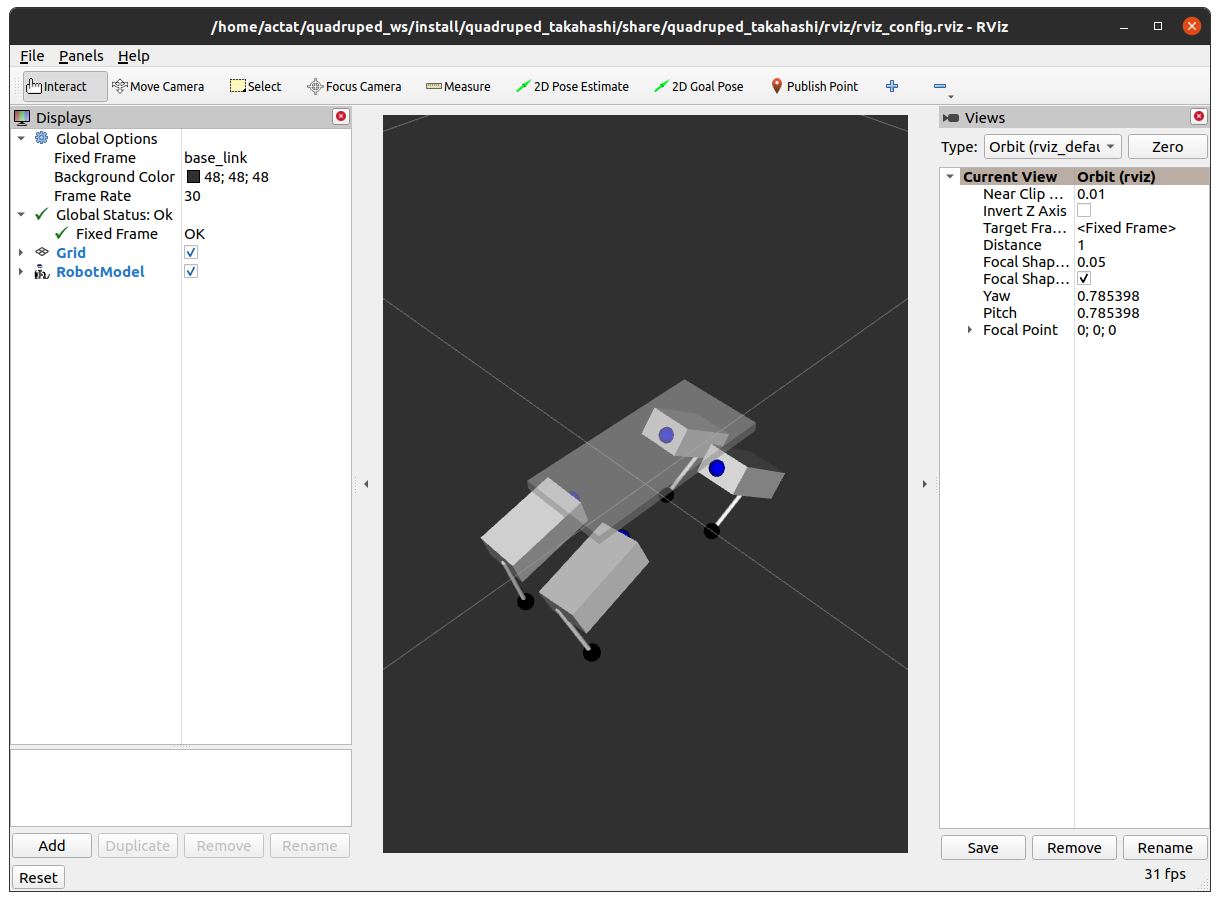
\includegraphics[width=15cm]{urdf_rviz_screen.png}
    \caption{URDFファイルを読み込んで表示するrvizの画面}
    \label{fig:urdf_rviz_screen}
  \end{figure*}

  \section{IMUのデータを読み取る}

  胴体中央下部に株式会社アールティのUSB出力9軸IMUセンサモジュールが搭載されている.
  rt-net/rt\_usb\_9axisimu\_driverによってrosのtopic(/imu/data\_rawと/imu/mag)にデータをパブリッシュする.
  パブリッシュされたデータはCCNYRoboticsLab/imu\_toolsのimu\_complementary\_filterで姿勢の情報にする.
  使用するパッケージをpackage.xmlに追記し,launchファイルにノードを起動する記述を追加した.

  \texttt{odom}から\texttt{base\_link}への\texttt{tf}をパブリッシュする
  \texttt{quadruped\_takahashi\_odometry\_node}というノードを作る.
  \texttt{/imu/data}をサブスクライブし,更新が入ったらコールバックで足の情報を参照して\texttt{tf}に情報を出す.
  ひとまず$xy$平面内での位置はゼロに固定し,高さは最も低い位置にある足が接地しているものとする.

  \section{脚の逆運動学}

  \texttt{base\_link}における足の位置を指令して各モータを追従させるために逆運動学計算を実装する.
  初めに,各関節がとれる値の範囲を表\ref{table:range_joint_angle}のとおりに定める.

  \begin{table}[htb]
    \caption{関節角の範囲}
    \label{table:range_joint_angle}
    \centering
    \begin{tabular}{rcccccc}
      \hline
      id & 脚 & 関節 & \multicolumn{2}{c}{最小値} & \multicolumn{2}{c}{最大値} \\
       &  &  & deg & rad & deg & rad \\
      \hline
      0 & 左前 & Hip ab/adduction & -10 & -0.174532925 & 45 & 0.785398163 \\
      1 & 左前 & Hip flexion/extension & -90 & -1.570796326 & 0 & 0 \\
      2 & 左前 & knee & 0 & 0 & 160.53 & 2.801777048 \\
      3 & 右前 & Hip ab/adduction & -45 & -0.785398163 & 10 & 0.174532925 \\
      4 & 右前 & Hip flexion/extension & -90 & -1.570796326 & 0 & 0 \\
      5 & 右前 & knee & 0 & 0 & 160.53 & 2.801777048 \\
      6 & 左後 & Hip ab/adduction & -10 & -0.174532925 & 45 & 0.785398163 \\
      7 & 左後 & Hip flexion/extension & 0 & 0 & 90 & 1.570796326 \\
      8 & 左後 & knee & -160.53 & -2.801777048 & 0 & 0 \\
      9 & 右後 & Hip ab/adduction & -45 & -0.785398163 & 10 & 0.174532925 \\
      10 & 右後 & Hip flexion/extension & 0 & 0 & 90 & 1.570796326 \\
      11 & 右後 & knee & -160.53 & -2.801777048 & 0 & 0 \\
      \hline
    \end{tabular}
  \end{table}

  初めに順運動学を考え,\texttt{base\_link}からみた各足の位置を表す
  ベクトル  $\boldsymbol{r}_\mathrm{xx4}^\mathrm{base}$を
  関節角$\theta_\mathrm{xx0}, \theta_\mathrm{xx1}, \theta_\mathrm{xx2}$を用いて表す.
  ここではxxは左前脚・右前脚・左後脚・右後脚に合わせてlf, rf, lh, rhが入るものとする.
  \texttt{base\_link}からみた脚の付け根の位置を表すベクトルを
  $\boldsymbol{r}^\mathrm{base}_\mathrm{xx0}$,
  腿と脛の長さを$l_\mathrm{t}, l_\mathrm{s}$とすると以下のようになる.
  \[
    \boldsymbol{r}_\mathrm{xx4}^\mathrm{base} = \boldsymbol{r}^\mathrm{base}_\mathrm{xx0} + \begin{bmatrix}
      -l_\mathrm{t}\sin{\theta_\mathrm{xx1}} - l_\mathrm{s}\sin{\left(\theta_\mathrm{xx1}+\theta_\mathrm{xx2}\right)} \\
      \sin\theta_\mathrm{xx0}\left(l_\mathrm{t}\cos{\theta_\mathrm{xx1}} + l_\mathrm{s}\cos{\left(\theta_\mathrm{xx1}+\theta_\mathrm{xx2}\right)}\right) \\
      -\cos\theta_\mathrm{xx0}\left(l_\mathrm{t}\cos{\theta_\mathrm{xx1}} + l_\mathrm{s}\cos{\left(\theta_\mathrm{xx1}+\theta_\mathrm{xx2}\right)}\right) \\
    \end{bmatrix}
  \]

  ここからは逆運動学を考える.
  脚の付け根の位置ベクトル$\boldsymbol{r}^\mathrm{base}_\mathrm{xx0}$は定数なので最初にこれを引いて
  $\boldsymbol{r}_\mathrm{xx4}^\mathrm{base} - \boldsymbol{r}^\mathrm{base}_\mathrm{xx0} = [x\, y\, z]^T$とする.

  初めに$y, z$のみで定まる$\theta_\mathrm{xx0}$を求める.
  $z\neq 0$の場合は以下の通り,$\arctan$で求められる.
  \begin{gather*}
    \left\{
    \begin{array}{l}
        y = \sin\theta_\mathrm{xx0}\left(l_\mathrm{t}\cos{\theta_\mathrm{xx1}} + l_\mathrm{s}\cos{\left(\theta_\mathrm{xx1}+\theta_\mathrm{xx2}\right)}\right) \\
        z = -\cos\theta_\mathrm{xx0}\left(l_\mathrm{t}\cos{\theta_\mathrm{xx1}} + l_\mathrm{s}\cos{\left(\theta_\mathrm{xx1}+\theta_\mathrm{xx2}\right)}\right)
      \end{array}
    \right. \\
    -\frac{y}{z} = \tan\theta_\mathrm{xx0} \\
    \theta_\mathrm{xx0} = \arctan{\left(-\frac{y}{z}\right)}
  \end{gather*}

  $z = 0$の場合,図\ref{fig:fig_ik_z0}に示すように$\theta_\mathrm{xx0}$は任意の値をとれる.
  便宜上,この場合は$\theta_\mathrm{xx0}=0$に定めることにする.

  \[
    \theta_\mathrm{xx0} = \begin{cases}
      0 & z = 0\text{のとき} \\
      \arctan{\left(-\frac{y}{z}\right)} & z\neq 0\text{のとき}
    \end{cases}
  \]

  \begin{figure*}[htb]
    \centering
    \input{fig_ik_z0.pdf_tex}
    \caption{
      $z = 0$の場合,$\theta_\mathrm{xx0}$は任意の値をとれる.
    }
    \label{fig:fig_ik_z0}
  \end{figure*}

  次に脚の長さに注目して膝関節の角度$\theta_\mathrm{xx2}$を求める.
  \begin{align*}
    x^2 + y^2 + z^2 &= \left|\boldsymbol{r}_\mathrm{xx4}^\mathrm{base} - \boldsymbol{r}^\mathrm{base}_\mathrm{xx0}\right|^2 \\
    &= \left(-l_\mathrm{t}\sin{\theta_\mathrm{xx1}} - l_\mathrm{s}\sin{\left(\theta_\mathrm{xx1}+\theta_\mathrm{xx2}\right)}\right)^2 \\
    &\quad + \left(\sin\theta_\mathrm{xx0}\left(l_\mathrm{t}\cos{\theta_\mathrm{xx1}} + l_\mathrm{s}\cos{\left(\theta_\mathrm{xx1}+\theta_\mathrm{xx2}\right)}\right)\right)^2 \\
    &\quad + \left(-\cos\theta_\mathrm{xx0}\left(l_\mathrm{t}\cos{\theta_\mathrm{xx1}} + l_\mathrm{s}\cos{\left(\theta_\mathrm{xx1}+\theta_\mathrm{xx2}\right)}\right)\right)^2 \\
    &= \left(-l_\mathrm{t}\sin{\theta_\mathrm{xx1}} - l_\mathrm{s}\sin{\left(\theta_\mathrm{xx1}+\theta_\mathrm{xx2}\right)}\right)^2 \\
    &\quad + \left(l_\mathrm{t}\cos{\theta_\mathrm{xx1}} + l_\mathrm{s}\cos{\left(\theta_\mathrm{xx1}+\theta_\mathrm{xx2}\right)}\right)^2 \\
    &= l_\mathrm{t}^2 + 2l_\mathrm{t}l_\mathrm{s}\left(
      \sin{\theta_\mathrm{xx1}}\sin{\left(\theta_\mathrm{xx1}+\theta_\mathrm{xx2}\right)}
      + \cos{\theta_\mathrm{xx1}}\cos{\left(\theta_\mathrm{xx1}+\theta_\mathrm{xx2}\right)}\right)
     + l_\mathrm{s}^2 \\
    &= l_\mathrm{t}^2 + 2l_\mathrm{t}l_\mathrm{s}\cos{\theta_\mathrm{xx2}} + l_\mathrm{s}^2 \\
    \cos{\theta_\mathrm{xx2}} &= \frac{x^2 + y^2 + z^2 - l_\mathrm{t}^2 - l_\mathrm{s}^2}{2l_\mathrm{t}l_\mathrm{s}}
  \end{align*}
  膝関節の値域は前脚の場合$0 \leq \theta_\mathrm{xf2} \leq 2.801777048$,後脚の場合$-2.801777048 \leq \theta_\mathrm{xh2} \leq 0$であることに注意する.
  \[
    \theta_\mathrm{xx2} = \begin{cases}
      \arccos{\frac{x^2 + y^2 + z^2 - l_\mathrm{t}^2 - l_\mathrm{s}^2}{2l_\mathrm{t}l_\mathrm{s}}} & \text{前脚の場合} \\
      -\arccos{\frac{x^2 + y^2 + z^2 - l_\mathrm{t}^2 - l_\mathrm{s}^2}{2l_\mathrm{t}l_\mathrm{s}}} & \text{後脚の場合}
    \end{cases}
  \]

  最後に$\theta_\mathrm{xx1}$を求める.
  $x$と$y^2+z^2$の式変形により,$\sin\theta_\mathrm{xx1}, \cos\theta_\mathrm{xx1}$の関係式を得る.
  \begin{align*}
    x &= -l_\mathrm{t}\sin{\theta_\mathrm{xx1}} - l_\mathrm{s}\sin{\left(\theta_\mathrm{xx1}+\theta_\mathrm{xx2}\right)} \\
    &= -l_\mathrm{t}\sin{\theta_\mathrm{xx1}}
    - l_\mathrm{s}\left(\sin\theta_\mathrm{xx1}\cos\theta_\mathrm{xx2} + \cos\theta_\mathrm{xx1}\sin\theta_\mathrm{xx2}\right) \\
    &= \left(- l_\mathrm{s}\sin\theta_\mathrm{xx2}\right)\cos\theta_\mathrm{xx1}
    + \left(-l_\mathrm{t}- l_\mathrm{s}\cos\theta_\mathrm{xx2}\right)\sin{\theta_\mathrm{xx1}}
  \end{align*}
  \begin{align*}
    y^2+z^2 &= \left(l_\mathrm{t}\cos{\theta_\mathrm{xx1}} + l_\mathrm{s}\cos{\left(\theta_\mathrm{xx1}+\theta_\mathrm{xx2}\right)}\right)^2 \\
    &= \left(l_\mathrm{t}\cos{\theta_\mathrm{xx1}}
    + l_\mathrm{s}\left(\cos\theta_\mathrm{xx1}\cos\theta_\mathrm{xx2} - \sin\theta_\mathrm{xx1}\sin\theta_\mathrm{xx2}\right)\right)^2 \\
    &= \left(\left(l_\mathrm{t} + l_\mathrm{s}\cos\theta_\mathrm{xx2}\right)\cos\theta_\mathrm{xx1}
    + \left(- l_\mathrm{s}\sin\theta_\mathrm{xx2}\right)\sin\theta_\mathrm{xx1}\right)^2
  \end{align*}
  値の範囲を確認する.
  前脚の場合$-1.570796326 \leq \theta_\mathrm{xf1} \leq 0, 0 \leq \theta_\mathrm{xf2} \leq 2.801777048$なので,
  $0 \leq \cos\theta_\mathrm{xf1} \leq 1, -1 \leq \sin\theta_\mathrm{xf1} \leq 0,
  -1 < \cos\theta_\mathrm{xf2} \leq 1, 0 \leq \sin\theta_\mathrm{xf2} \leq 1$である.
  今,$l_\mathrm{t} = l_\mathrm{s}$なので
  $\left(l_\mathrm{t} + l_\mathrm{s}\cos\theta_\mathrm{xf2}\right)\cos\theta_\mathrm{xf1} \geq 0,
  \left(- l_\mathrm{s}\sin\theta_\mathrm{xf2}\right)\sin\theta_\mathrm{xf1} \geq 0$だから
  \[
    \sqrt{y^2+z^2} = \left(l_\mathrm{t} + l_\mathrm{s}\cos\theta_\mathrm{xf2}\right)\cos\theta_\mathrm{xf1}
    + \left(- l_\mathrm{s}\sin\theta_\mathrm{xf2}\right)\sin\theta_\mathrm{xf1}
  \]
  である.
  後脚の場合$0 \leq \theta_\mathrm{xh1} \leq 1.570796326, -2.801777048 \leq \theta_\mathrm{xh2} \leq 0$なので,
  $0 \leq \cos\theta_\mathrm{xh1} \leq 1, 0 \leq \sin\theta_\mathrm{xh1} \leq 1,
  -1 < \cos\theta_\mathrm{xh2} \leq 1, -1 \leq \sin\theta_\mathrm{xh2} \leq 0$である.
  $l_\mathrm{t} = l_\mathrm{s}$だから
  $\left(l_\mathrm{t} + l_\mathrm{s}\cos\theta_\mathrm{xh2}\right)\cos\theta_\mathrm{xh1} \geq 0,
  \left(- l_\mathrm{s}\sin\theta_\mathrm{xh2}\right)\sin\theta_\mathrm{xh1} \geq 0$なので
  \[
    \sqrt{y^2+z^2} = \left(l_\mathrm{t} + l_\mathrm{s}\cos\theta_\mathrm{xh2}\right)\cos\theta_\mathrm{xh1}
    + \left(- l_\mathrm{s}\sin\theta_\mathrm{xh2}\right)\sin\theta_\mathrm{xh1}
  \]
  である.結局前脚でも後脚でも
  \[
    \sqrt{y^2+z^2} = \left(l_\mathrm{t} + l_\mathrm{s}\cos\theta_\mathrm{xx2}\right)\cos\theta_\mathrm{xx1}
    + \left(- l_\mathrm{s}\sin\theta_\mathrm{xx2}\right)\sin\theta_\mathrm{xx1}
  \]
  である.
  これで$\sin\theta_\mathrm{xx1}, \cos\theta_\mathrm{xx1}$の1次式を2つ得られたので,連立して値を求められる.
  \begin{align*}
    \begin{bmatrix} x \\ \sqrt{y^2 + z^2} \end{bmatrix} &=
    \begin{bmatrix}
      - l_\mathrm{s}\sin\theta_\mathrm{xx2} & -l_\mathrm{t}- l_\mathrm{s}\cos\theta_\mathrm{xx2} \\
      l_\mathrm{t} + l_\mathrm{s}\cos\theta_\mathrm{xx2} & - l_\mathrm{s}\sin\theta_\mathrm{xx2}
    \end{bmatrix}
    \begin{bmatrix} \cos\theta_\mathrm{xx1} \\ \sin\theta_\mathrm{xx1} \end{bmatrix} \\
    \begin{bmatrix} \cos\theta_\mathrm{xx1} \\ \sin\theta_\mathrm{xx1} \end{bmatrix}
    &= \frac{1}{l_\mathrm{t}^2 + 2l_\mathrm{t}l_\mathrm{s}\cos\theta_\mathrm{xx2} + l_\mathrm{s}^2}
    \begin{bmatrix}
      - l_\mathrm{s}\sin\theta_\mathrm{xx2} & l_\mathrm{t} + l_\mathrm{s}\cos\theta_\mathrm{xx2} \\
      -l_\mathrm{t} - l_\mathrm{s}\cos\theta_\mathrm{xx2} & - l_\mathrm{s}\sin\theta_\mathrm{xx2}
    \end{bmatrix}
    \begin{bmatrix} x \\ \sqrt{y^2 + z^2} \end{bmatrix} \\
    \tan\theta_\mathrm{xx1} &= \frac{\sin\theta_\mathrm{xx1}}{\cos\theta_\mathrm{xx1}} \\
    &= \frac{x\left(-l_\mathrm{t} - l_\mathrm{s}\cos\theta_\mathrm{xx2}\right) + \sqrt{y^2 + z^2}\left(-l_\mathrm{s}\sin\theta_\mathrm{xx2}\right)}
    {x\left(-l_\mathrm{s}\sin\theta_\mathrm{xx2}\right) + \sqrt{y^2 + z^2}\left(l_\mathrm{t} + l_\mathrm{s}\cos\theta_\mathrm{xx2}\right)} \\
    \theta_\mathrm{xx1} &= \arctan\left(
      \frac{x\left(-l_\mathrm{t} - l_\mathrm{s}\cos\theta_\mathrm{xx2}\right) + \sqrt{y^2 + z^2}\left(-l_\mathrm{s}\sin\theta_\mathrm{xx2}\right)}
      {x\left(-l_\mathrm{s}\sin\theta_\mathrm{xx2}\right) + \sqrt{y^2 + z^2}\left(l_\mathrm{t} + l_\mathrm{s}\cos\theta_\mathrm{xx2}\right)}
    \right)
  \end{align*}

  以上まとめると\texttt{base\_link}からみた各足の位置を表すベクトル$\boldsymbol{r}_\mathrm{xx4}^\mathrm{base}$から関節角を以下の手順で求められる.
  \begin{itemize}
    \item 脚の付け根の位置ベクトル$\boldsymbol{r}^\mathrm{base}_\mathrm{xx0}$を引いて
    $[x\, y\, z]^T = \boldsymbol{r}_\mathrm{xx4}^\mathrm{base} - \boldsymbol{r}^\mathrm{base}_\mathrm{xx0}$とする.
    \item $\theta_\mathrm{xx0} = \mathrm{atan2}\left(y, -z\right)$
    \item $\theta_\mathrm{xx2} = \begin{cases}
      \arccos{\frac{x^2 + y^2 + z^2 - l_\mathrm{t}^2 - l_\mathrm{s}^2}{2l_\mathrm{t}l_\mathrm{s}}} & \text{前脚の場合} \\
      -\arccos{\frac{x^2 + y^2 + z^2 - l_\mathrm{t}^2 - l_\mathrm{s}^2}{2l_\mathrm{t}l_\mathrm{s}}} & \text{後脚の場合}
    \end{cases}$
    \item $\theta_\mathrm{xx1} = \mathrm{atan2}\left(
      \frac{x\left(-l_\mathrm{t} - l_\mathrm{s}\cos\theta_\mathrm{xx2}\right) + \sqrt{y^2 + z^2}\left(-l_\mathrm{s}\sin\theta_\mathrm{xx2}\right)}
      {l_\mathrm{t}^2 + 2l_\mathrm{t}l_\mathrm{s}\cos\theta_\mathrm{xx2} + l_\mathrm{s}^2},
      \frac{x\left(-l_\mathrm{s}\sin\theta_\mathrm{xx2}\right) + \sqrt{y^2 + z^2}\left(l_\mathrm{t} + l_\mathrm{s}\cos\theta_\mathrm{xx2}\right)}
      {l_\mathrm{t}^2 + 2l_\mathrm{t}l_\mathrm{s}\cos\theta_\mathrm{xx2} + l_\mathrm{s}^2}
    \right)$
  \end{itemize}

  逆運動学計算を実装する.
  脚の付け根の関節角$\theta_\mathrm{xx0}, \theta_\mathrm{xx1}$は$\mathrm{atan2}$であり,引数両方がゼロの時にエラーになる可能性がある.
  $\theta_\mathrm{xx0}$で引数両方がゼロになるのは$y = z = 0$のときで,この時は$\theta_\mathrm{xx0} = 0$とすることに決めていた.
  $\theta_\mathrm{xx1}$は$\theta_\mathrm{xx1} = \pi$になって脚の長さがゼロにならない限り問題は起こらない.
  $\theta_\mathrm{xx2}$は$\boldsymbol{r}_\mathrm{xx4}^\mathrm{base} - \boldsymbol{r}^\mathrm{base}_\mathrm{xx0}$の長さによって定義域を外れる.
  脚の長さが長すぎるときは最大限に伸展した状態になるように例外処理を入れる.

\section{ロボットに指令を送る方法}

ロボットの制御に関連する処理は\texttt{quadruped\_takahashi\_control\_node}の処理として実装する.
ロボットが行うべき操作(モータの制御モードを切り替える・姿勢を変える・歩行する)を外部から指令する仕組みが必要である.
そこで入力が文字列で真理値と文字列を返すサービス\texttt{quadruped\_takahashi\_control\_node/mode}がある.
入力文字列に応じて処理を行い,問題なければ\texttt{true}を返す.
問題がある場合は\texttt{false}と問題点を文字列で返す.

サービスのコールバックには\texttt{void quadruped\_takahashi\_control\_node::callback\_mode\_(...)}が設定されている.
この関数は
\begin{itemize}
  \item 前のモードを解除
  \item 入力の文字列に対応する関数の呼び出し
\end{itemize}
を行う.
呼び出される関数は\texttt{void quadruped\_takahashi\_control\_node::mode\_\{\text{文字列}\}\_(...)}としてある.
サービスはノードの起動時に立ち上がるようにしてある.

launchファイルによってノードを起動したら別のウインドウを開いてサービスを呼べる.
例えば,モータをfreeするときは\texttt{ros2 service call /quadruped\_takahashi\_control\_node/mode quadruped\_takahashi/srv/Mode "\{'data': 'motor\_free'\}"}とする.

\end{document}
